
\subsection*{\textbf{Question 1.c)}}
\begin{quote}

\textbf{Problem}
\begin{quote}
Write a code that can do the KS-test on the your function to determine if it is consistent with a normal distribution. For this, use $\mu = 0$ and $\sigma = 1$. Make a plot of the probability that your Gaussian random number generator is consistent with Gaussian distributed random numbers, start with 10 random numbers and use in your plot a spacing of 0.1 dex until you have calculated it for $10^5$ random numbers on the x-axis. Compare your algorithm with the KS-test function from \texttt{scipy, scipy.stats.kstest} by making an other plot with the result from your KS-test and the KS-test from scipy.
\end{quote}

\textbf{Solution} 
\begin{quote}
The implementation of the KS-test is in general straight forwards. There are however two points of interest that needs to be discussed. The first point is the implementation of the CDF for the KS-statistic and the second point is the implementation of the CDF for the normal distribution.
\\

\textbf{(1) CDF KS-statistic }
\begin{quote}
The p-value produced by the KS-tests requires the evaluation of the CDF for the KS-test statistic,
\begin{equation}
P_{KS}(z) = \frac{2\sqrt{\pi}}{z} \sum_{j=1}^{\infty} \exp\left(- \frac{(2j-1)^2+\pi^2}{8z^2} \right)
\end{equation}

This infinite sum needs to be numerically approximated in order to perform the KS-test. The chosen approximation for the above equation is taken from the book \textit{Numerical Recipes - The art of Scientific Computation, 3d edition}, 

\begin{equation}
P_{KS}(z) \approx
\begin{cases}
\frac{\sqrt{2 \pi}}{z} \left[ \left( e^{-\pi^2/(8z^2)} \right)+^{9} + \left( e^{-\pi^2/(8z^2)} \right) \left( e^{-\pi^2/(8z^2)} \right)^{25} \right] &\quad \text{for $ z < 1.18$}\\
1 -2 \left[ \left(e^{-2z^2}\right) - \left(e^{-2z^2}\right)^4 + \left(e^{-2z^2}\right)^9 \right]  &\quad \text{for $ z >= 1.18$}
\end{cases}
\end{equation}
\end{quote}

\textbf{(2) CDF normal distribution}
\begin{quote}
The CDF of the normal distribution is needed in order to perform the KS-test under the null hypothesis that the data follows a normal distribution. The CDF of the normal distribution can in general be written as,
\begin{equation}
\Phi\left( \frac{x- \mu}{\sigma}\right) = \frac{1}{2} \left[ 1 + \text{erf} \left( \frac{x - \mu}{\sigma\sqrt{2}} \right) \right]
\end{equation}

where the erf is given by,
\begin{equation}
\text{erf}(x)  \frac{2}{\sqrt{\pi}} \int_0^{x} e^{-t^2} dt
\end{equation}

The integral of the erf function lacks a closed form and therefore needs to be numerically approximated. The chosen approximation is taken from \textit{Abramowitz and Stegun},

\begin{equation}
\text{erf}(x) \approx 1- (a_1t+a_2t^2 + ... + a_5t^5)e^{-x^2} \text{x} \quad t = \frac{1}{1+px}
\end{equation}

where, $p  =0.3275911$, $a_1 =  0.254829592$, $a_2 = -0.284496736$, $a_3 = 1.421413741$, $a_4 =  -1.453152027$, $a_5 = 1.061405429$.
\end{quote}

The KS-test and the CDF are implemented with these approximations. The code for the KS-test and the CDF  is located in the file \texttt{./Code/mathlib/statistics.py} at page 22, as this file is threaded as a shared module. The KS-test does require an sorting algorithm, this algorithm is implemented in the file \texttt{./Code/matlib/sorting} and can be found on page 26. 
 The code for the generation of the plots and plots are displayed below.  
\end{quote}

\newpage
\textbf{Code - Plots}

\begin{quote}
The code for generating the two plots. The imports for this file are not explicit shown, but can be found on page 19.
\lstinputlisting[firstline=124,lastline=180]{./Code/assigment_1.py}
\end{quote}
\newpage

\textbf{Code - Output plot(s)}
\begin{quote}
\begin{figure}[!ht]
\centering
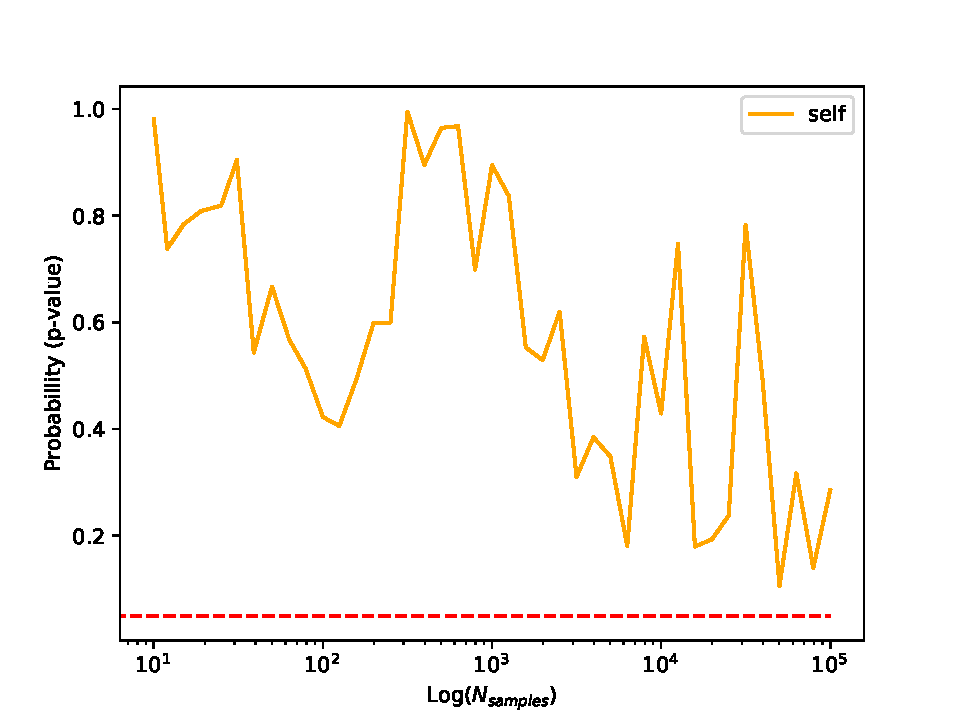
\includegraphics[width=12cm, height=7.5cm]{./Plots/1_plot_ks_test_self.pdf}
\caption{The P-value produced by the KS-test against the number of samples on which the KS-test is performed for the self written RNG. The red line indicates the line of $ p = 0.05$. A point \textbf{below} the line would suggests that there is enough statistical evidence to reject the (null) hypothesis that the data is normal distributed. The plot shows that the RNG always passes KS-test up to atleast $10^5$ samples. The p-value  does however appear to drop for a large number of samples and might even drop further when more samples are used. The drop suggests again that the RNG is likely not perfect.}
\end{figure}

\begin{figure}[!hb]
\centering
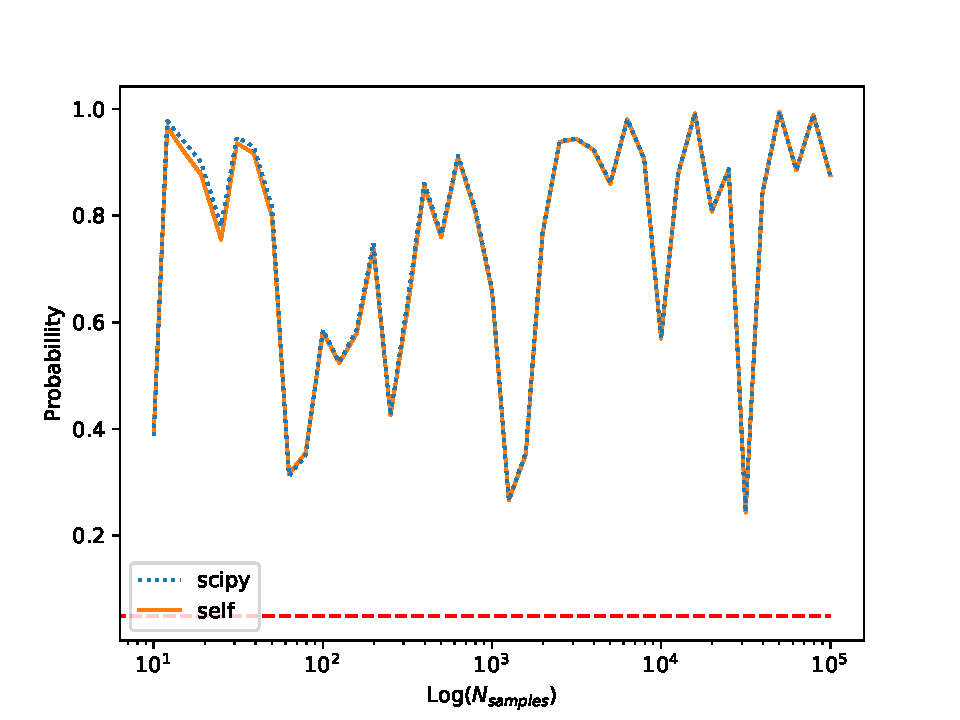
\includegraphics[width=12cm, height=7.5cm]{./Plots/1_plot_ks_test_self_scipy.pdf}
\caption{The P-value produced by the KS-test against the number of samples on which the KS-test is performed for the self written RNG. The red line indicates the line of $ p = 0.05$. The orange line is the self written implementation of the KS-test and the blue line is the scipy version.  A point \textbf{below} the red line would suggests that there is enough statistical evidence to reject the (null) hypothesis that the data is normal distributed. The self written KS-test is  close to the scipy version, but shows (small) deviations at small sample sizes (see $N_{samples} = 10$ or $N_{samples} = 200$).  The self written implementation always has the same shape as the scipy version, even at the deviations. The exact cause for the deviations are unknown, but are likely the result of an approximation that scipy makes that the self written implementation doesn't make. }
\end{figure}
\end{quote}

\end{quote}



%\textbf{Code - output } 
%\begin{quote}
% The code that produces the output.
%\lstinputlisting{./code/assigment1_a.py}
%\end{quote}

%\textbf{Code - helper } 
%\begin{quote}
%The code for the Poisson distribution and the factorial function.  
%\lstinputlisting[firstline=2,lastline=46]{./code/mathlib/utils.py}
%\end{quote}


%\textbf{Output}
%\begin{quote}
%The output produced by \textsf{/code/assigment1\_ a.py} 
%\lstinputlisting{./output/assigment1_a_out.txt}
%\end{quote}











